\documentclass[a4paper,twosides]{report}
\usepackage[utf8]{inputenc}
\usepackage{lmodern}
\usepackage[T1]{fontenc}
\usepackage[italian]{babel}
\usepackage{microtype}
\usepackage{acronym}
\usepackage{mathtools}
\usepackage{amsfonts}
\usepackage{amsthm}
\usepackage[hidelinks,breaklinks=true]{hyperref}
\usepackage{xcolor}
\usepackage{listings}

\newcommand{\me}{\ensuremath{\mathrm{e}}}
\newcommand{\md}{\ensuremath{\mathrm{d}}}
\newcommand{\tc}{\ensuremath{\mathrm{t.c.:}\quad}}
\newcommand{\expected}[1]{\ensuremath{\mathrm{\textbf{E}}\left[#1\right]}}
\newcommand{\variance}[1]{\ensuremath{\mathrm{\textbf{Var}}\left(#1\right)}}
\newcommand{\prob}[1]{\ensuremath{\mathrm{\textbf{P}}\left(#1\right)}}
%\newcommand{\max}[1]{\ensuremath{\mathrm{max}\left(#1\right)}}
\newcommand{\abs}[1]{\ensuremath{\left|#1\right|}}
\newcommand{\mR}{\ensuremath{\mathbb{R}}}
\newcommand{\codei}[1]{\texttt{#1}}

\newtheorem{defi}{Definizione}[chapter]

\lstset{inputpath=src}
\lstdefinestyle{customPy}{
 language=python,
 showstringspaces=false,
 basicstyle=\footnotesize\ttfamily,
 keywordstyle=\bfseries\color{green!40!black},
 commentstyle=\itshape\color{purple!40!black},
 identifierstyle=\color{blue},
 stringstyle=\color{orange},
}

%\DeclarePairedDelimiter\abs{\lvert}{\rvert}

\author{
  {\Large Stefano Martina}\\
  {\small stefano.martina@stud.unifi.it}\\
  Universit\`a degli Studi di Firenze\\
  Scuola di Scienze Matematiche, Fisiche e Naturali\\
  Corso magistrale di Informatica
}
\title{{\Huge\bfseries Cenni di fisica statistica}\\{\large\bfseries
    Esame di Laboratorio di Fisica Computazionale}}

\begin{document}
\maketitle
\thispagestyle{empty}
\vfill
\begin{abstract}
  Questo lavoro presenta una breve introduzione alla fisica
  statistica.
\end{abstract}
\clearpage
\acresetall

\graphicspath{{img/}}

\chapter{\acf{LMM} e \acf{LRM}}
In questo capitolo vengono presi in considerazione due metodi che
permettono di calcolare in modo semplice la soluzione a problemi
di massimizzazione o minimizzazione di funzioni multivariate
sottoposte a vincoli. Ad esempio problemi come quello di trovare il
punto più elevato di una strada di campagna (massimizzare la funzione
bivariata che rappresenta l'elevazione del terreno sottoposta al
vincolo rappresentato dalla strada), oppure trovare il punto di minima
pressione all'interno del perimetro regionale (minimizzare la funzione
bivariata che rappresenta la carta delle isobare sottoposta al vincolo
dato dai confini della regione).
\section{\acf{LMM}}
Il \ac{LMM} \`e una strategia che permette di trovare il massimo o il
minimo di una funzione sottoposta a vincoli dati da
equazioni. \`E utile analizzare prima il caso con un solo vincolo.
\subsection{Singolo vincolo}
Viene indicato con $f$ la funzione da
massimizzare/minimizzare e con $g$ il vincolo, per semplificare il
problema viene mostrato il caso in due variabili in cui:
\begin{eqnarray*}
f&:&\mR^2\rightarrow\mR\\
g&:&\mR^2\rightarrow\mR.
\end{eqnarray*}
Senza perdere generalit\`a viene preso in considerazione il problema
in cui \`e necessario massimizzare $f$, quindi formalmente il problema
\`e:
\begin{defi}
  \begin{eqnarray*}
    &&\max_{x,y}\left\{f(x,y)\right\}\\
    &&\tc{}\\
    &&\quad g(x,y)=0.
  \end{eqnarray*}
\end{defi}
Per applicare il metodo \`e necessario che $f$ e $g$ siano derivabili
alle prime derivate parziali in $x$ e $y$.

L'intuizione del metodo \`e quella di trovare i punti critici in cui
non \`e possibile aumentare $f$ nell'intorno della $g$.
\section{\acf{LRM}}
\chapter{\acf{MCM}}
  Questo capitolo presenta una breve introduzione al \acf{MCM}. Vengono
  mostrati inizialmente alcuni concetti di probabilit\`a necessari per
  le dimostrazioni, in seguito vi sono la dimostrazione e lo schema
  generale del \ac{MCM} ed infine viene mostrata una applicazione
  pratica del metodo, ossia come sia possibile ottenere una
  approssimazione dell'integrale definito di una funzione.
\section{Note sulla probabilit\`a}
\subsection{Errore probabile}
Per una variabile casuale $X$ distribuita normalmente con
\begin{itemize}
\item media $\mu$;
\item varianza $\sigma$;
\end{itemize}
si ha che per
\begin{equation*}
  r = 0.6745\sigma
\end{equation*}
vale
\begin{eqnarray*}
  \prob{\mu-r<X<\mu+r} &=& 0.5\\
  \prob{\abs{X-\mu}<r} &=& 0.5\\
  \prob{\abs{X-\mu}>r} &=& 0.5.
\end{eqnarray*}
Quindi valori di $X$ che deviano da $\mu$ pi\`u o meno di $r$ hanno
stesse probabilit\`a ed $r$ identifica l'errore pi\`u probabile di
una distribuzione normale.

\subsection{Teorema del limite centrale delle probabilit\`a}
Si considerino $N$ variabili casuali $X_1,X_2,\dots,X_N$ indipendenti e distribuite
identicamente. Quindi con stessa media e stessa varianza:
\begin{eqnarray*}
  \expected{X_1}=\expected{X_2}=\dots=\expected{X_N}&=&m\\
  \variance{X_1}=\variance{X_2}=\dots=\variance{X_N}&=&b^2.
\end{eqnarray*}

Si consideri la somma di queste variabili casuali:
\begin{equation*}
  Y = X_1+X_2+\cdots+X_N
\end{equation*}
si ha che
\begin{eqnarray*}
  \expected{Y}&=&\expected{X_1+X_2+\cdots+X_N}=Nm\\
  \variance{Y}&=&\variance{X_1+X_2+\cdots+X_N}=Nb^2.
\end{eqnarray*}

Si consideri adesso una variabile casuale $Z$ distribuita normalmente
con parametri:
\begin{eqnarray*}
  \mu&=&Nm\\
  \sigma&=&b\sqrt{N}
\end{eqnarray*}
con funzione di densit\`a denotata da $p_Z(x)$.

Il teorema centrale del limite afferma che per $N$ grande, e per ogni
intervallo $(x_1,x_2)$ vale:
\begin{equation}\label{eq:tcl}
  \prob{x_1<Y<x_2}\approx\int_{x_1}^{x_2}p_Z(x) \md x
\end{equation}
quindi la somma di un numero elevato di variabili
casuali aventi distribuzione identica \`e distribuita normalmente con
media e varianza uguali a quelle originali (anche se queste non erano
distribuite normalmente).

\section{\acf{MCM}}
Supponendo di dover calcolare una certa quantit\`a sconosciuta $m$,
dobbiamo trovare una variabile casuale $X$ tale che:
\begin{equation*}
  \expected{X} = m.
\end{equation*}
Avendo tale distribuzione, con varianza uguale a:
\begin{equation*}
  \variance{X} = b^2
\end{equation*}
 \`e possibile mostrare i seguenti passaggi.

Si considerino $N$ variabili casuali $X_1,X_2,\dots,X_N$ con
distribuzione identica a quella di $X$. Quindi per il teorema del
limite centrale~\eqref{eq:tcl} si ha, per $N$ sufficientemente grande, che la
distribuzione della somma
\begin{equation*}
  Y=X_1+X_2+\cdots+X_N
\end{equation*}
\`e distribuita normalmente con parametri
\begin{eqnarray*}
  \mu &=& Nm\\
  \sigma&=&b\sqrt{N}.
\end{eqnarray*}

Per la regola dei \emph{tre sigma} si ha:
\begin{eqnarray*}
  \prob{\mu-3\sigma < Y <\mu +3\sigma}&\approx& 0.997\\
  \prob{Nm-3b\sqrt{N} < Y < Nm+3b\sqrt{N}}&\approx& 0.997
\end{eqnarray*}
dividendo per $N$:
\begin{eqnarray*}
  \prob{m-\frac{3b}{\sqrt{N}} < \frac{Y}{N} <
    m+\frac{3b}{\sqrt{N}}}&\approx& 0.997\\
  \prob{\abs{\frac{Y}{N}-m} <\frac{3b}{\sqrt{N}}}&\approx& 0.997
\end{eqnarray*}
e quindi:
\begin{equation}\label{eq:mc}
  \prob{\abs{\frac{1}{N}\sum_{i=1}^NX_i-m} <\frac{3b}{\sqrt{N}}}\approx 0.997.
\end{equation}

L'equazione~\eqref{eq:mc} afferma che, se viene estratto un campione per ogni
variabile casuale $X_i$, la media aritmetica di questi valori \`e
approssimativamente uguale a $m$. Inoltre, l'errore di questa
approssimazione \`e pari a $3b/\sqrt{N}$, che tende a $0$ al crescere
di $N$. \`E possibile ridurre ulteriormente l'incertezza
aumentando il numero $k$ di sigma usati per l'approssimazione e
quindi valutando l'errore $kb/\sqrt{N}$.

In realt\`a, poich\'e le variabili casuali $X_i$ hanno la stessa
distribuzione di $X$, \`e sufficiente estrarre $N$ campioni da $X$ per
giungere alle stesse conclusioni.
Il \ac{MCM} \`e costituito
dal seguente procedimento da adattare secondo i casi:
\begin{enumerate}
\item si trova la distribuzione $X$ con media la quantit\`a desiderata
  $m$ e varianza $b^2$;
\item si estraggono $N$ campioni di $X$, in numero grande abbastanza
  da avere un errore piccolo a piacere;
\item la media aritmetica di tali $N$ campioni d\`a il valore
  approssimato di $m$.
\end{enumerate}
Quindi il problema diventa quello di ricavare la distribuzione $X$ o,
comunque, gli $N$ campioni distribuiti in accordo con $X$.

Se vogliamo caratterizzare pi\`u nel dettaglio l'errore commesso
prendendo $N$ campioni, possiamo ricorrere all'\emph{errore
  probabile}. Ponendo $k=0.6745$ si ha che 
\begin{equation*}
  \prob{\abs{\frac{1}{N}\sum_{i=1}^NX_i-m} <\frac{0.6745\cdot b}{\sqrt{N}}}\approx 0.5
\end{equation*}
e quindi 
\begin{equation*}
  r_N = \frac{0.6745\cdot b}{\sqrt{N}}
\end{equation*}
 indica di quanto si discosta mediamente il
valore della media dei campioni $\frac{1}{N}\sum_{i=1}^NX_i$ dalla misura cercata
$m$. Tale valore caratterizza l'errore assoluto
\begin{equation*}
\abs{\frac{1}{N}\sum_{i=1}^NX_i-m}  
\end{equation*}
commesso prendendo $N$ campioni.

\subsection{\acf{MCI}}
Il \ac{MCM} \`e utile per simulare fenomeni che hanno un alto grado di
incertezza negli input o un alto numero di gradi di libert\`a.

Una
applicazione specifica \`e \ac{MCI}. Integrare numericamente una
funzione che ha
molte dimensioni o che ha caratteristiche particolari, come quella di
figura~\ref{fig:func}, pu\`o diventare un problema estremamente
difficile. Monte Carlo pu\`o essere utile in questi casi per ottenere
un'approssimazione dell'integrale.
\begin{figure}[h!]
  \centering
  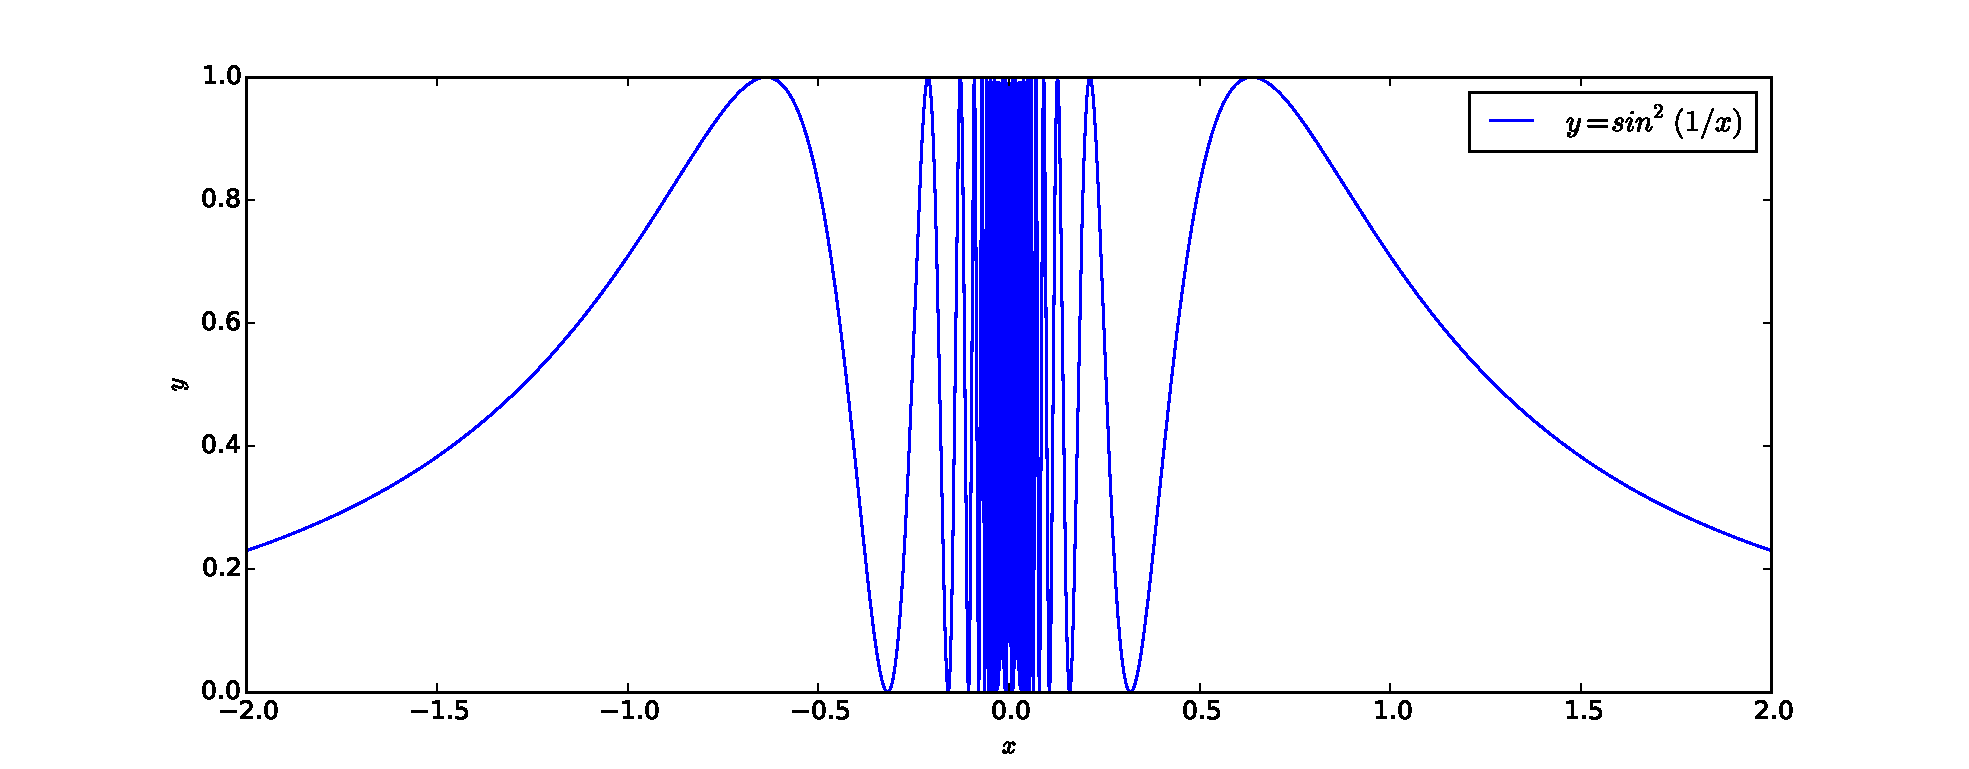
\includegraphics[width=\textwidth]{montecarlo1.pdf}
  \caption{Funzione $y=sen^2(1/x)$ non ben definita intorno allo $0$.}
  \label{fig:func}
\end{figure}

Consideriamo la funzione:
\begin{equation*}
  f(x)\equiv sen^2(\frac{1}{x}),
\end{equation*}
\`e sempre compresa tra $0$ e $1$, non \`e definita per
$x=0$ e inoltre intorno allo $0$ si addensano le oscillazioni. La
funzione integrale
\begin{equation*}
  I(x) \equiv \int_0^x f(x') \md x'
\end{equation*}
\`e l'area sotto la curva $f(x)$ compresa tra $0$ e $x$. Ha sempre valore finito
compreso tra $0<I(x)<X$, ma non \`e semplice da calcolare vicino
all'origine.

Se scegliamo due numeri casuali
\begin{itemize}
\item  $u$ uniformemente distribuito tra $0$ e $x$;
\item $v$ uniformemente distribuito tra $0$ e $1$;
\end{itemize}
si ha che la probabilit\`a che il punto $h = (u, v)$, nella
figura~\ref{fig:func}, sia sotto la curva 
$f(x)$ \`e $I(x)/x$, ossia il rapporto tra l'area sotto la curva e
l'area limitata da $0$ e $x$ nelle
ascisse e da $0$ e $1$ nelle ordinate.

Il punto $h$ \`e sotto la
curva se $v<f(u)$. Quindi, prendendo un campione sufficientemente
grande di $N$ punti e contando gli $M$ punti che stanno sotto la
curva\footnote{Usando la disequazione $v<f(u)$.}, \`e possibile
stimare il valore di $I(x)$ con:
\begin{equation*}
  I(x)\approx \frac{M}{N}x.
\end{equation*}

In figura~\ref{fig:int} \`e possibile vedere l'approssimazione di
$I(x)$ usando \ac{MCI} con $10000$ campioni. In appendice \`e
riportato il codice\footnote{Notare che le figure
  sono state create impostando \codei{numCampioni} e \codei{numPuntiX}
  uguali a 10000, mentre nel codice sono uguali a 1000 per velocizzare
  il processo in caso di esecuzione di questo.} \emph{Python} usato
per creare i plot delle
figure~\ref{fig:func} e~\ref{fig:int}.
\begin{figure}[h!]
  \centering
  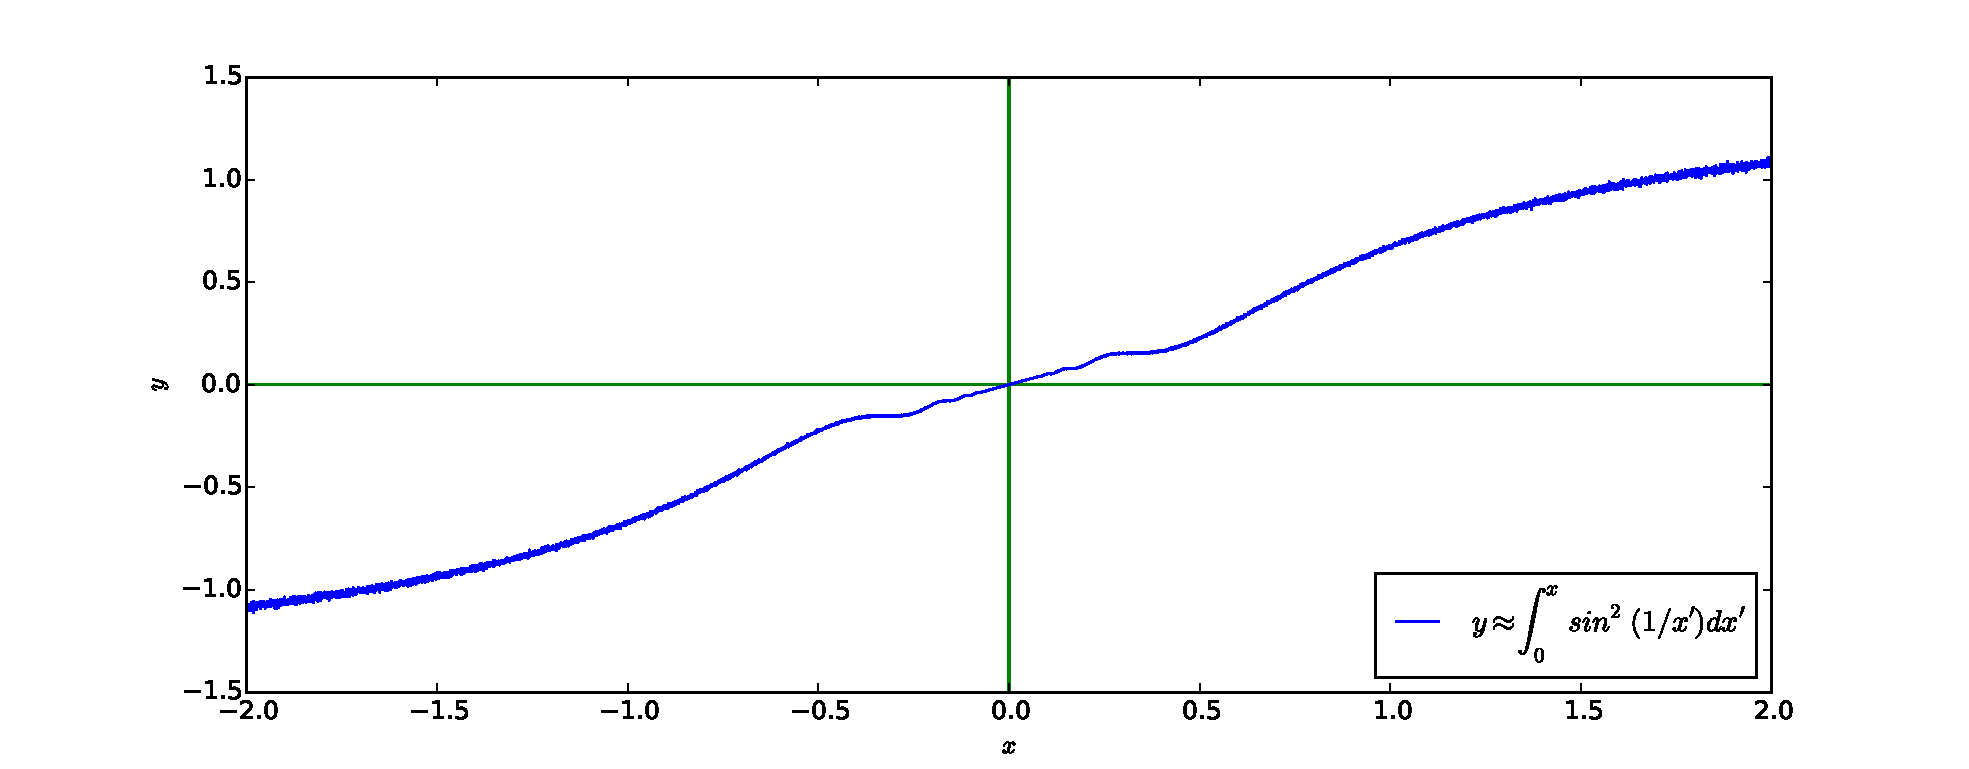
\includegraphics[width=\textwidth]{montecarlo2.pdf}
  \caption{Approssimazione della funzione integrale $y=\int_0^x sen^2(1/x')\md x'$, ottenuta
    con \ac{MCI} con $N=10000$ campioni.}
  \label{fig:int}
\end{figure}

\newpage
\section{Appendice}
\lstinputlisting[style=customPy]{montecarlo.py}


\chapter{\acf{SA}}
  Questo capitolo presenta una breve introduzione alla tecnica del
  \acf{SA} usata per trovare il massimo o minimo di una
  funzione. Vengono mostrate le origini del metodo e i parallelismi
  con la termodinamica statistica, in seguito viene introdotto il
  problema \acf{TSP} e mostrato un algoritmo che risolve il problema
  usando \ac{SA}.
\section{Introduzione}
Il \ac{SA} \`e un metodo usato per trovare l'ottimo globale di una
funzione data, si ispira ad un metodo usato in metallurgia chiamato
annealing che consiste nello scaldare e raffreddare lentamente un
materiale per aumentarne la dimensione dei cristalli e migliorarne le
caratteristiche chimico-fisiche.

La funzione da ottimizzare pu\`o avere diverse variabili, un tipico
esempio di problema per il quale pu\`o essere usato \ac{SA} \`e
\ac{TSP}.

\section{Termodinamica statistica}
Per descrivere i principi base della termodinamica statistica si
considera un sistema di esempio. In un reticolo monodimensionale ogni
punto \`e una particella con un valore di spin che pu\`o essere
\emph{up} o
\emph{down}. Se il reticolo ha $N$ punti, allora il sistema pu\`o
essere in $2^N$ diverse configurazioni, ad ognuna di queste
configurazioni corrisponde un valore di energia, ad esempio:
\begin{equation*}
  E=B(n_+-n_-)
\end{equation*}
dove $B$ \`e una certa costante, $n_+$ \`e il numero di particelle con
spin 
\emph{up}, ed $n_-$ \`e il numero di particelle con spin \emph{down}.

La probabilit\`a $P(\sigma)$ di trovare il sistema in una certa
configurazione
$\sigma$ \`e data dalla distribuzione di Boltzmann-Gibbs:
\begin{equation}\label{eq:distBoltz}
  P(\sigma) = C \me^{-E_\sigma/T}
\end{equation}
dove $E_\sigma$ \`e l'energia della configurazione, $T$ \`e la
temperatura\footnote{Nella distribuzione di Boltzmann-Gibbs al
  denominatore dell'esponente vi \`e $kT$ dove $k$ \`e la costante di
  Boltzmann e $T$ \`e la temperatura termodinamica. Ma per l'esempio
  la temperatura \`e un parametro svincolato dalla realt\`a fisica
  quindi \`e possibile trascurare $k$.} e $C$ \`e una costante di
normalizzazione.

L'energia media del sistema in equilibrio \`e quindi:
\begin{eqnarray*}
  \bar{E} &=& \frac{\sum_\sigma E_\sigma P(\sigma)}{\sum_\sigma
    P(\sigma)}\\
  &=& \frac{\sum_\sigma E_\sigma \me^{-E_\sigma/T}}{\sum_\sigma \me^{-E_\sigma/T}}
\end{eqnarray*}
Calcolare numericamente il valore di $\bar{E}$ pu\`o essere
difficile al crescere del numero degli stati, per\`o \`e possibile
creare un algoritmo di Monte Carlo che simula le fluttuazioni casuali
tra gli stati in modo che la distribuzione data
dall'equazione~\eqref{eq:distBoltz} sia rispettata. Partendo da una
configurazione iniziale arbitraria, dopo un certo numero di \emph{trial} di Monte
Carlo il metodo converge verso lo stato di
equilibrio $\bar{E}$ e continua ad oscillare intorno ad $\bar{E}$.

\ac{SA} \`e un metodo di questo tipo.

\section{Algoritmo \acf{SA}}
Il \ac{SA} si muove su un sistema partendo da un certo stato iniziale
$s_0$, quindi esegue una serie di iterazioni nelle quali viene
valutato un vicino dello stato e, con una certa distribuzione di
probabilit\`a, la dinamica si sposta nel nuovo stato vicino o meno.

Un possibile codice \emph{c-style} di un metodo \ac{SA} \`e il seguente:
\begin{lstlisting}[frame=single, numbers=left, language=C]
s = s0;
for(int k=0; k<kMax; ++k) {
  T = temp(k/kMax);
  sNew = vicino(s);
  if (random(0,1) < P(E(s), E(sNew), T)) {
    s = sNew;
  }
}
return s;
\end{lstlisting}
In riga \codei{1} viene inizializzato il ciclo con lo stato iniziale
\codei{s0}, in seguito vi \`e un ciclo che esegue \codei{kMax}
iterazioni. In riga \codei{3} viene assegnato un certo
valore di tempo a \codei{T} che dipende dal progresso delle
iterazioni. In riga \codei{4} viene scelto casualmente un vicino \codei{sNew} dello
stato \codei{s}. In riga \codei{5} vi \`e il fulcro dell'algoritmo,
\codei{random} sceglie uniformemente un numero casuale in $[0,1)$ e
\codei{P} implementa la distribuzione di probabilit\`a di accettazione
che dipende dall'energia
misurata in \codei{s}, da quella in \codei{sNew} e dalla temperatura
\codei{T}. In caso di accettazione viene preso \codei{sNew} come nuovo
stato di base e continua il processo.

La relazione con la termodinamica statistica sta nel fatto che
\codei{P} viene scelta in modo da mantenere vera la
relazione~\eqref{eq:distBoltz}\footnote{\`E sufficiente che siano relazioni simili.},
inoltre il metodo \codei{temp} ritorna
valori decrescenti di temperatura al crescere delle iterazioni, da qui
il paragone con l'annealing in metallurgia.

Originalmente, per
rispettare i principi della termodinamica statistica, \codei{P} venne
scelta in modo da ritornare \codei{1} se
$E(sNew)<E(s)$ e $\me^{-(E(sNew)-E(s))/T}$ altrimenti. Tale
condizione non \`e strettamente necessaria per realizzare dei metodi
\ac{SA}.

\section{\acf{TSP}}
\ac{TSP} \`e un problema di ottimizzazione combinatoria e verr\`a
usato come esempio per descrivere il metodo \ac{SA}. Vengono dati:
\begin{itemize}
\item una lista di $N$ citt\`a identificate dai naturali da $1$ ad $N$;
\item una matrice $D$, $N\times N$, dove $D_{i,j}$ \`e la distanza, o
  costo, per andare dalla citt\`a $i$ alla citt\`a $j$;
\item si indica con $\{x_i\}_1^N$ una permutazione $x$ dei naturali da
  $1$ a $N$, ovvero delle citt\`a.
\end{itemize}
L'obbiettivo del problema \`e di trovare una permutazione $c$ delle
citt\`a tale che sia minima la distanza $d$ espressa dall'equazione:
\begin{equation}\label{eq:distanzaTSP}
  d(c) = D_{c_N,c_1}+\sum_{k=1}^{N-1}D_{c_k,c_{k+1}}
\end{equation}

Ossia si chiede di trovare un percorso che:
\begin{enumerate}
\item passi da tutte le citt\`a
  una ed una sola volta;
\item sia ciclico, ossia finisca nella citt\`a da cui \`e cominciato;
\item sia quello con lunghezza minima tra quelli che rispettano le due
  precedenti condizioni.
\end{enumerate}

\section{Soluzione \acf{TSP} con \acf{SA}}
Per risolvere il problema \ac{TSP} vengono interpretati come stati le
diverse permutazioni delle $N$ citt\`a e viene interpretata la distanza data
dalla formula~\eqref{eq:distanzaTSP} come energia del sistema quando
si trova in un certo stato, ossia permutazione delle citt\`a.
Lo pseudo codice che implementa il metodo \`e il seguente:
\begin{lstlisting}[frame=single, numbers=left]
tsp(s, T) {
  c[k] = s[k] per k=1,...,N
  dc = distanza(c)
  i = 1
  while (! stop()) {
    j = random(1,N) diverso da i
    t = scambia(c, i, j)
    dt = distanza(t)
    if ((dt<dc) or (random(0,1)<exp((dc-dt)/T))) {
      c[k] = t[k] per k=1,...,N
      dc = dt
    }
    i = modulo(i, N) + 1
  }
  return c
}
\end{lstlisting}
dove il metodo \codei{distanza(s)} calcola la distanza di un percorso
rappresentato da una permutazione \codei{s}:
\begin{lstlisting}[frame=single, numbers=left]
distanza(s) {
  return D[s[N],s[1]] + sum(D[s[k], s[k+1]])
                             per k=1,...,N-1
}
\end{lstlisting}
\codei{scambia(c, i, j)} scambia \codei{i} con \codei{j} nel
percorso \codei{c} e inverte la direzione di quelli in mezzo a
\codei{i} e \codei{j}:
\begin{lstlisting}[frame=single, numbers=left]
scambia(c, i, j) {
  a = min(i,j)
  b = max(i,j)
  t[k] = c[k]      per k=1,...,a-1
  t[a+k] = c[b-k]  per k=0,...,b-a
  t[k] = c[k]      per k=b+1,...,N
  return t
}  
\end{lstlisting}
\codei{i = modulo(i,N)+1} serve per iterare \codei{i} in $1,\dots,N$
ripetutamente.

Nel codice visto manca da definire la condizione di stop
data dal metodo \codei{stop()}, essa dovrebbe avvenire quando viene
raggiunto un equilibrio, ossia quando il metodo oscilla intorno ad un
certo stato. L'idea \`e che inizialmente si lancia
la procedura con uno stato iniziale \codei{s} casuale e con una
temperatura \codei{T} casuale o scelta con un certo criterio. L'algoritmo si ferma
quando viene raggiunto un equilibrio e ritorna lo stato \codei{c} in
quell'equilibrio. A questo punto viene decrementato opportunamente la
temperatura
\codei{T} e viene eseguita nuovamente la procedura chiamandola sui due nuovi valori
\codei{TSP(c,T)}.


\chapter*{Acronimi}
\addcontentsline{toc}{section}{Acronimi}
\begin{acronym}[MCM]
  \acro{LMM}{Lagrange Multipliers Method}
  \acro{LRM}{Lagrange Relaxation Method}
  \acro{MCI}{Monte Carlo Integration}
  \acro{MCM}{Monte Carlo Method}
  \acro{SA}{Simulated Annealing}
  \acro{TSP}{Traveling Salesman Problem}
\end{acronym}

\nocite{*}
\phantomsection
\addcontentsline{toc}{section}{\refname}
\bibliographystyle{apalike}
\bibliography{elaborato}

\end{document} 
